\documentclass[acmsmall,screen,review,anonymous]{acmart}

%%
%% \BibTeX command to typeset BibTeX logo in the docs
\AtBeginDocument{%
  \providecommand\BibTeX{{%
    Bib\TeX}}}

%% Rights management information.  This information is sent to you
%% when you complete the rights form.  These commands have SAMPLE
%% values in them; it is your responsibility as an author to replace
%% the commands and values with those provided to you when you
%% complete the rights form.
\setcopyright{acmcopyright}
\copyrightyear{2018}
\acmYear{2018}
\acmDOI{XXXXXXX.XXXXXXX}


%%
%% Submission ID.
%% Use this when submitting an article to a sponsored event. You'll
%% receive a unique submission ID from the organizers
%% of the event, and this ID should be used as the parameter to this command.
%%\acmSubmissionID{123-A56-BU3}

\usepackage{listings}

\lstdefinestyle{mystyle}{
  basicstyle=\ttfamily\footnotesize,
  breakatwhitespace=true,
  breaklines=true,
  keepspaces=true,
  showspaces=false,
  showstringspaces=false,
  showtabs=false,
  tabsize=2,
  captionpos=b
}
\lstset{style=mystyle}
\usepackage{graphicx}
\usepackage{caption}

\begin{document}

\title{Bridging the Gap Between Visual and Analytical Machine Learning Testing}

\author{Anon}

\begin{abstract}
% what is the problem?
% why is this an important problem to solve?
% what did we do?
% what did we find?
Testing ML systems is a highly interactive process which demands a human-in-the-loop approach. In addition to writing tests for the code base, practitioners are required to analyse and interpret several visualisations using their domain expertise to validate if an ML system satisfies the required set of functional and non-functional properties. Visualisations are frequently used to qualitatively assess various parts of an ML pipeline. However, implicit knowledge gained from visualisations must be translated to explicit analytical tests that fail when there is change in any component of the ML pipeline. We conduct an empirical analysis of Jupyter notebooks to catalogue the state-of-the- art mappings between ML visualisations and assertions. We mine Github to collect Jupyter Notebooks that contain assertions written in Python. We develop a novel methodology to identify 1764 notebooks which contain an assertion below a visualisation. We manually analyse the 1.7K notebooks and identify 551 notebooks where at least one pair of visualisation and assertion are semantically related to one another. We further read and understand 90 notebooks in depth to identify 26 qualitative and their corresponding quantitative testing patterns. We showcase five such patterns in this paper and plan to make the entire catalogue publicly available in the near future.

\end{abstract}

\maketitle

\section{Introduction}\label{sec:intro}
% what problem are we trying to solve?
% what is our motivation here?

% NOTE our methodology of finding visualisation and assertion that are related is a (pretty good) contribution.

\section{Preliminaries}\label{sec:prelim}
\subsection{ML Testing}\label{sec:ml-testing}
% zhang2020machine

% The emphasis is primarily on image datasets and DNNs, specifically
% CNNs & RNNs. Almost all papers are vested in the notion of addressing
% qualitative metrics such as robustness, safety & privacy. Of these 3
% robustness appears most frequently because it is the easiest to define
% in terms of quantitative metrics.

% The two most common domains are safety-critical systems (such as
% autonomous driving) & neural machine translation (NMT)
% [ji2021automated, sun2020automatic, he2020structure].

% The proposed testing techniques can be classified into 4
% categories:

% 1. Improvements over existing test adequacy metrics such as neuron
%    coverage which was proposed by DeepExplore & DeepGauge
%    [gerasimou2020importance].
% 2. Formal verification methods which try to provide formal guarantee
%    of robustness against adversarial examples [zhu2021deepmemory,
%    baluta2021scalable].
% 3. Data augmentation techniques which generate adversarial examples to
%    be used during training to improve robustness of models. There are
%    techniques based on fuzzing & seach based software testing
%    (SBST) [braiek2019deepevolution, gao2020fuzz] and mutation testing
%    [wang2021robot, zhang2020white].
% 4. And finally some papers propose adversarial detection during
%    runtime [xiao2021self, wang2020dissector, wang2019adversarial,
%    berend2020cats].


\subsection{Computational Notebooks and Software
  Engineering}\label{sec:notebooks}

% NOTE maybe this should be about jupyter notebook mining and work
% done? Then we can say that these are the only two publicly available
% datasets with notebooks; and the challenges we faced when trying to
% use them!

% TODO review Kastner's bib, he also has a section dedicated to prior
% work done using notebooks!

% TODO we need to defend why we did not use kgtorrent dataset for our analysis. We can say that we performed analysis on random samples of notebooks from kaggle and did not find that many interesting examples?

% TODO some form of introduction to the notion of computational notebooks; literal programming?

Computational notebooks have been ubiquitously adopted by the machine learning community for developing ML enabled systems. Although originally intended to promote reproducible software, computational notebooks are infamous for the exact opposite since they do not follow software engineering best practices.

The process of understanding and cleaning the underlying training data---commonly referred to as "data wrangling"---tends to dominate the ML development workflow~\cite{CITME}. Data wrangling is high iterative. Practitioners often explore several hypotheses, visual designs, methods, tools, algorithms and data sources to arrive at the final implementation. Studies have been conducted to understand how practitioners generate, evaluate and manage such alternatives. ~\cite{liu2019understanding,kandel2012enterprise}.

Developing software in computational notebooks introduces a new paradigm for writing code. In addition to code, notebooks also contain additional information in the form of natural language text and images. To better understand the process of working within computational notebooks and the challenges faced along the way, studies with human subjects have been conducted\cite{head2019managing}.


 ML practitioners often experiment with several versions of code to implement the same functionality. Prior work has explored how practitioners manage the different versions of code and the challenges that they face along the way.

\citeauthor{quaranta2021kgtorrent} mine Kaggle~\footnote{https://kaggle.com} and present \textit{KGTorrent}, a public dataset consisting of approximately 2.5 million Jupyter notebooks written in Python. The dataset also contains a relational database dump of metadata regarding publicly available notebooks on Kaggle. The KGTorrent dataset is publicly available on Zenodo, in the form of a 81TB compressed file.


% TODO yang2021subtle: data scientists spend most of their time preparing the data ('data wrangling'). Authors propose WrangleDoc, a tool that automatically generates documentation of data wrangling code and what effect it has on the data. They integrate their tool with JupyterLab and evaluate using 100 notebooks from Kaggle and also with practitioners.

% code quality; reproducibility; best practices...
\citeauthor{pimentel2019large} mine 1.4 million notebooks from Github to conduct an empirical study on the good and bad coding practices when developing software using computational notebooks. The authors also make their dataset of notebooks publicly available on Zenodo~\footnote{https://zenodo.org/record/2592524}. Computational notebooks were originally designed to promote sharing reproducible research since they allow presenting information by interweaving natural text, code and other multimedia such as tables, images and videos. However, the authors discover that Jupyter notebooks are far from being reproducible due to bad coding practices such as lack of separation of concern, testing and versioning.

% TODO psallidas2019data: paper conducts a super massive empirical study: 6M python notebooks from github, 2M enterprise DS pipelines (anonymous company name), source code and metadata from 900+ releases 12 important DS libraries. Paper provides high-level guidelines on what technologies DS practitioners should focus and what system builders should focus on to serve practitioners better.

% TODO head2019managing: notebooks do not follow best practices. authors typically work in an iterative fashion, often experimenting with different versions of code to analyse data and produce meaningful visualisations. This leads to duplicates and messy notebooks. The paper presents a code gathering tool that allows notebook authors to review various versions and only keep the relevant version. Paper performs qualitative usability study using 12 participants.

% TODO kery2018story: study with 21 participants on coding practices when working in notebooks. Authors observe that practitioners often have multiple versions that lead to problems and reduced readability. Participants typically create narative through order of cells rather than with the use of markdown cells. Paper then conducts survey with 45 data scientists and provides design guidelines for future literate programming tools.

% TODO chattopadhyay2020wrong: semi-structed interviews (n=20) and survey (n=156) to understand pain points when working with notebooks. Guidelines on design of computational notebooks.


% DONE kandel2012enterprise: semi-structured interview study (n=35) with data analysts from 25 organizations across diverse sectors. Relationship between data analysis and how oganizational features of enterprise affect it. Recurring painpoints, open challenges and guidelines for building better visual analysis research.

% DONE liu2019understanding: semi-structed interview study (n=12) with data workers with various expertise and domain knowledge. Paper wants to understand the process behind exploring "alternatives": different hypothesis, visual design, methods, tools, algorithms, data sources. The studies explores the motivation behind exploring such alternatives, how alternatives help with sense making process, high-level process of alternatives and how practitioners generate, explore and manage such alternatives.

computational notebooks have been widely adopted by the data science and machine learning community for developing ML models. Unlike traditional software, ML enabled systems evolve through change in not only the code base, but also the complexity of the model and the underlying training data.

Naturally, research is active in understanding the process of developing using notebooks. Prior work has looked into best practices
\subsection{Visualisations and Machine Learning}\label{sec:visualisations}

% TODO bavishi2021vizsmith: paper presents VizSmith, an automatic
% data visualisation framework that accepts data in the form of pandas
% dataframe along with a list of columns the user wishes to visualise.
% The tool then automatically produces visualisations for the
% specified columns.

% TODO amershi2015modeltracker: model building is a cognitively
% disruptive step; practitioners are required to iterate between model
% building and error analysis. Paper presents ModelTracker, a
% visualisation tool that presents all the information in traditional
% summary statistics along with the performance of the model. Tool
% validated with users who used the tool for 6 months in a production
% setting.

% TODO gortler2022neo: Research with ML practitioners at Apple and
% identify traditional confusion matrix does not support complex data
% structures that are prevalent today. Paper proposes Neo, an
% interactive and multi-output confusion matrix.

% TODO yang2022pattern: Paper conducts study on interaction techniques for Multivariate matrix visualisations.

% TODO wang2023gam: paper proposes GAM COACH, a tool that generates customizable counterfactual explanations for Generalized Additive Models (GAMs). The tools uses interactive visualisations to allow users to iteratively generate algorithmic recourse plans. The tool is qualitatively validated by users(n=41).

% TODO ahn2023escape: paper proposes ESCAPE, a visual analytics tool that allows users to identify systematic errors in AI enabled systems. The tool promotes a human-in-the-loop approach to identify spurious associations and concept associated misclassifications.

% TODO wang2023drava: paper proposes DRAVA, a visual analytics tool to relate human concepts with semantic dimensions extracted by ML models during Disentangled representation learning>. The tool also provides feedback to minimize the mismatches and helps practitioners obtain data insights fron concept-driven exploration. The tool is validated using application scenarios in an experimental setting.

% TODO robertson2023angler: authors propose ANGLER, a visual analytics tools to help practitioners prioritise machine translation model improvements. Tool is validated with machine translation experts (n=7). The tool allows users to validate interesting hypotheses for prioritising model improvements.

% TODO bernard2019visual: paper proposes visual-analytics tool to perform data pre-processing of multi-variate time series data.

% TODO gschwandtner2018know: paper proposes visual analytics technique to perform data profiling of time series data

% TODO yuan2021survey: survey of visual analytics techniques used in ML. Paper proposes taxonomy of visual analytics techniques: before model building, during model building and after model building.

% TODO wexler2020if: paper proposes WHAT-IF tool, a model agnostic, interactive visualisation tool the understanding ML models. The tool allows users to visually analyse and verify their hypothesis regarding the training data and how the model works. The tool requires a trained model and a sample dataset. The tool is integrated with Tensorflow, Jupyter and Collaboratory notebooks. The tool allows conterfactual reasoning, investigate decision boundariesa and investigate how change in data affects the prediction.

% TODO hohman2019visual: survey of visual analytics techniques specifically for deep learning models. Visual analytics has been rapidly used for model explanation, interpretation, debugging and improvement.


\subsection{Technical Background}\label{sec:background}
\subsubsection{Internal Structure of Jupyter Notebooks}\ref{sec:nbformat}
% TODO we need to explain the json structure of jupyter notebooks, we reference this in the methodology to explain the github query.

\lstinputlisting[]{nbformat.json}
\captionof{lstlisting}{Internal JSON structure of Jupyter Notebooks.}
\label{lst:nbformat}

The data comprised within Jupyter Notebooks is stored in the JSON format, and thus can be parsed programmatically. Listing~\ref{lst:nbformat} shows the internal json structure of Jupyter Notebooks, adopted from the official nbformat website.~\footnote{https://nbformat.readthedocs.io/en/latest/index.html}. For simplicity, we only show the parts that are relevant for this study.

Notebooks contain four top level keys namely \texttt{metadata}, \texttt{nbformat}, \texttt{nbformat\_minor} and \texttt{cells}. The \texttt{matadata} key consists of additional information regarding the notebook such as the kernel and programming language. \texttt{nbformat} and \texttt{nbformat\_minor} contain the version of nbformat used in the notebook. The \texttt{cells} key consists of a list of all cells within the notebook.

Listing~\ref{lst:nbformat} presents three examples of cells. Each cell is represented as a dictionary with the \texttt{cell\_type}, \texttt{metadata} and \texttt{source} keys. Cells can be of three types: "markdown", "code" or "raw". The contents of each cell can be found within the \texttt{source} key, as a list of strings.

The output generated by a code cell is stored within the \texttt{outputs} key. Static visualisations are stored as base64 encoded png images under the \texttt{"image/png"} key, which is nested within the \texttt{data} key inside \texttt{outputs}. Since a cell can generate multiple outputs, the \texttt{outputs} key is a list.

\subsubsection{Pre and Post-Condition Checks}\ref{sec:pre-post-cond}
% TODO explain and give examples of what we mean by pre/post-condition checks with examples

% TODO contrast this to the type of tests we are actually looking for! Why are pre/post conditions not valuable to look at?

\section{Methodology}\label{sec:method}
% TODO is there a scientific term in SE research to explain reading code in detail?
% NOTE we looked for semantic similarity between the visualisation and assertion code

This section presents the methodology used to conduct the empirical
study presented in Section~\ref{sec:intro}. Figure~\ref{fig:method}
presents an overview of all relevant steps used in this study. The
empirical analysis comprises of three distinct phases namely:
\textit{the data collection phase}, \textit{identification of related
visualisation and assertion pairs} and finally a \textit{complete
analysis of the notebooks} to identify the final set of 29
visualisation and assertion pairs.

The yellow boxes in the data collection phase represent filters that
were applied to the 54K notebooks obtained from Gihub, to obtain the
final sample size of 1.7K notebooks used in the empirical study. The red
boxes represent the exclusion criteria used during phase two to remove
notebooks note relevant for this study. Finally, the green boxes in
phase 3 represent the manual analysis conducted to identify the final 29
visualisation and assertion pairs.

Boxes appearning next to one-another imply that they were applied
using an "OR" operator. While boxes appearning below one-another imply
an "AND" operator. Text in double quotes represent the string pattern
used in the search query.

More details regarding each phase of the methodology is presented below.

% TODO update the numbers
\begin{figure}
  \centering
  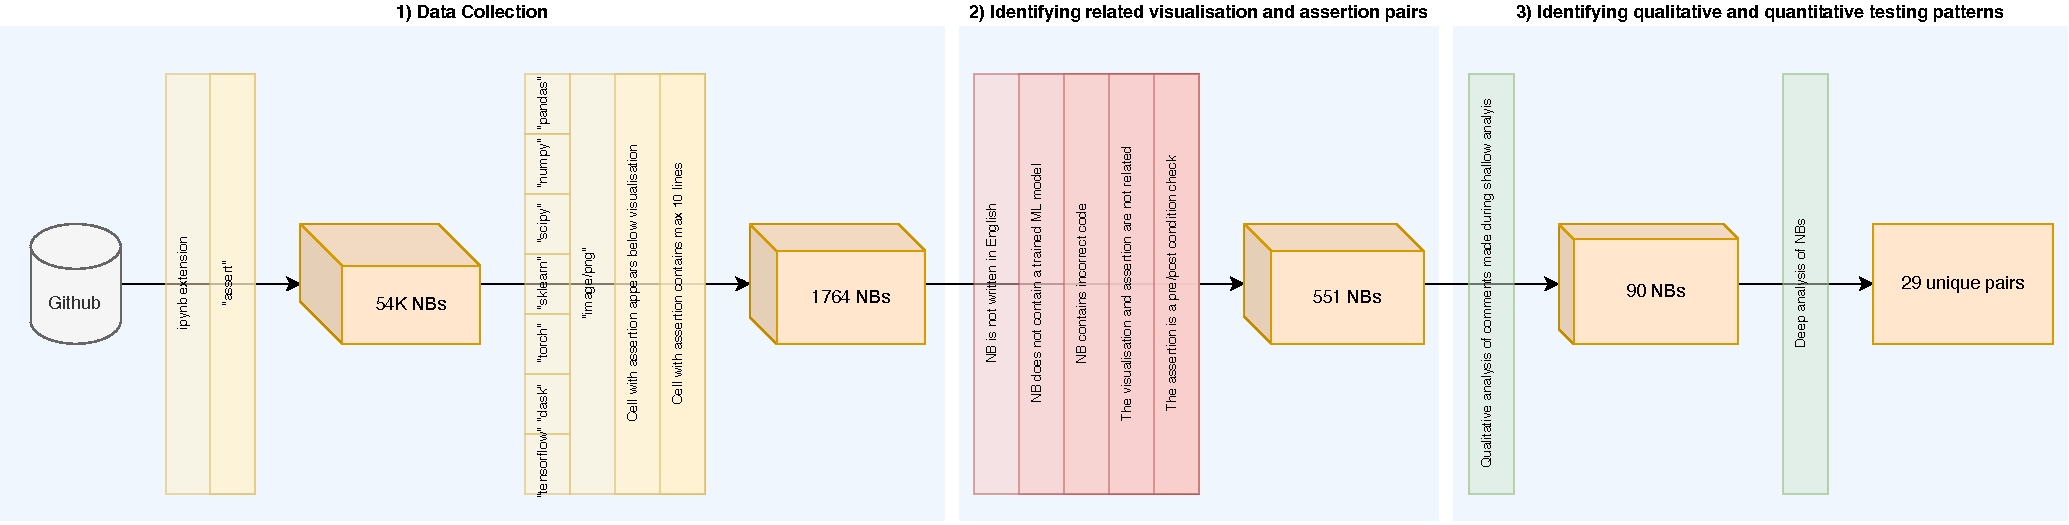
\includegraphics[width=\textwidth]{method.pdf}
  \caption{Methodology used to collect and analyse Jupyter notebooks
    in this study.}
  \label{fig:method}
\end{figure}

\subsection{Data Collection}\label{sec:data-collect}

We mined public repositories from Github to collect Jupyter
notebooks---files with the \texttt{.ipynb} extension---that contain
the keyword ``assert'' in them.

% TODO is it clear what I am trying to say here?
% FIXME is "testing statement" the right terminology?

We intentionally keep the search criteria on Github broad by only
checking for the appropriate filetype and the presence of the
``assert'' keyword. This is because, the ``assert'' keyword is used in
python to define tests. Additionally, popular python libraries which
provide a testing interface (such as nose, unittest and numpy),
contain the same keyword in their API. Thus, our search criteria
captures a large initial sample of $54,070$ notebooks with a variety
of testing statements. Our approach also prevents the need to craft a
custom search query based on an exhaustive list of keywords that
appear in all python testing libraries.

\begin{table}
  \centering
  \caption{Filters used during data collection phase.}
  \begin{tabular}{l p{0.4\textwidth} p{0.4\textwidth}}
    \toprule
    \textbf{ID} &
    \textbf{Filter} &
    \textbf{Rationale}\\
    \midrule
    \emph{\textbf{F1}} &
    Files with extension \texttt{.ipynb} &
    This translates to the following Github search query:
    \texttt{filename:"Jupyter Notebook"}.\\
    \emph{\textbf{F2}} &
    Notebooks with \texttt{"assert"} keyword &
    \texttt{"assert"} is used in python to define tests. Additionally,
    it also appears in other python libraries which provide their own
    testing interface.\\
    \emph{\textbf{F2}} &
    Notebooks with popular data science or machine learning libraries &
    The list of python libraries is derived by performing a web search
    along with the author's prior knowledge and expertise in ML. We
    combine the patterns using an \texttt{"OR"} operator. The final
    regex pattern is the following:
    \texttt{"tensorflow"|"dask"|"torch"|"sklearn"
    |"scipy"|"numpy"|"pandas"}.\\
    \emph{\textbf{F3}} &
    Notebooks that contain visualisations &
    Section~\ref{sec:nbformat} describes the internal son structure
    of Jupyter notebooks. Visualisations are stored as binary strings
    under the \texttt{"image/png"} field.\\
    \emph{\textbf{F4}} &
    Notebooks where the assertion appears below the visualisation &
    The code cell containing the assertion must be defined below the
    cell that produces the visualisation. Any number of markdown cells
    may appear between the visualisation and assertion cells. See
    Section~\ref{sec:cell-arrangement} for detailed explanation.\\
    \emph{\textbf{F5}} &
    Notebooks where the assertion cell is not longer than 10 lines &
    The code cell containing the assertion should not be longer than
    10 lines. The threshold for max lines was derived based on our
    observations from a random sample of 50 notebooks. See
    Section~\ref{sec:cell-arrangement} for detailed explanation.\\
    \bottomrule
  \end{tabular}
  \label{tab:filters}
\end{table}

Table~\ref{tab:filters} summarises the filters used during the data
collection phase to obtain the final sample of 1.7K notebooks from the
initial sample of 54K notebooks mined from Github. The table provides
a short description of the filter along with our rationale for using
them.

% TODO don't mention quantity of random sample; then we need to explain/defend this choice
We used an iterative approach to determine the effectiveness of each
filter that was used. We applied each filter in the same order as
presented in Table~\ref{tab:filters}, starting with F1. We randomly
sampled 50 notebooks from the population of notebooks obtained after
applying the filter. We then conduct the qualitative assessment
presented in Section~\ref{REFME} and observe the number of related
visualisation and assertion pairs. In each new iteration, we
progressively add the other filters and include the filter if the
number of relevant visualisation and assertion pairs increases.

% TODO maybe use colors from red-green to denote arrangements that produced better results? (instead of binary)
\begin{figure}
  \centering
  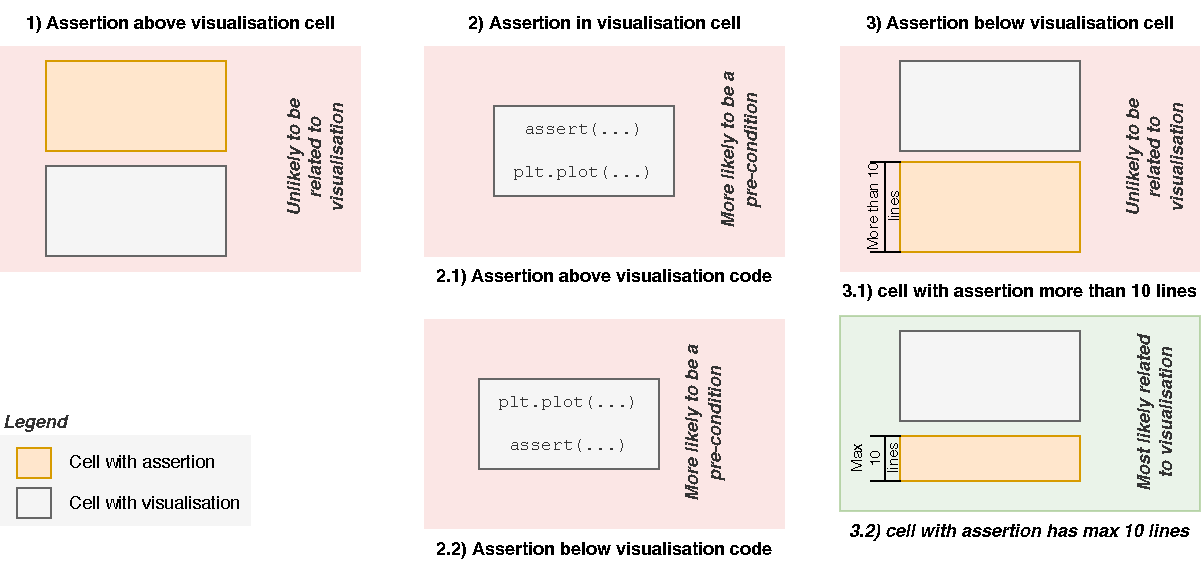
\includegraphics[width=\textwidth]{nb-structure.pdf}
  \caption{Arrangement of code cells containing assertion and
    visualisation.}
  \label{fig:cell-arrangement}
\end{figure}

For RQ1, we are interested in finding empirical evidence of visualisations and corresponding assertions used in the wild. To answer this question, we further reduce our notebook sample size by assuming a specific order in which the visualisation and assertion code cells appear in the notebooks. Figure~\ref{fig:cell-arrangement} presents a visual representation of various arrangements of code cells that may occur in notebooks. Note that the visual representation omits markdown cells since we only consider the order of code cells in our analysis. In the actual notebook however, one or more markdown cells may be present between the visualisation and assertion cells.

As explained above, the selected arrangement of code cells was discovered by qualitatively analysing a random sample of notebooks with the code cell arrangements presented in Figure~\ref{fig:cell-arrangement}. We observed the signal-to-noise ratio for each cell arrangement. And picked the arrangement with the least signal-to-noise ratio. Table~\ref{tab:cell-arrangement} summarises our observations from the various cell arrangements.

% TODO give more examples (from our data) of what a pre/post condition check is
\begin{table}
  \centering
  \caption{Observations from random samples of notebooks with various
  cell arrangement.}
  \begin{tabular}{l p{0.4\textwidth} p{0.4\textwidth}}
    \toprule
    \emph{\textbf{ID}}&
    \emph{\textbf{Cell arrangement}} &
    \emph{\textbf{Observations}}\\
    \midrule
    1 &
    Assertion above visualisation cell &
    The assertions in this arrangement were typically not related to the visualisation below. Often, a markdown cell present between the assertion and visualisation code cells, would mark the begining of a new section in the notebook. In other cases, the assertions were typically pre-condition checks to ensure that the visualisation code would not encounter any errors. Pre-condition checks typically include checking the shape of features that are used in the visualisation. Or checking that the length of the ``x''and ``y`` features are the same to ensure a continuous line in the plot.\\
    2.1 &
    Assertion in the visualisation cell: assertion above visualisation code &
    Our observations were similar to that of arrangement 1. the assertions defined above the visualistion code were more likely to be pre-condition checks.\\
    2.2 &
    Assertion in the visualisation cell: assertion below visualisation code &
    We found several examples where the assertion was related to the visualisation. Most often however, the assertions were post-condition checks to ensure the correctness of the visualisation itself. The signal-to-noise ratio in this arrangement was also higher compared to arrangement 3.2.\\
    3.1 &
    Assertion below visualisation cell: assertion cell more than 10 lines &
    The assertions in this arrangement were frequently related to the visualisation above. In some cases, a markdown cell between the visualisation and assertion marked the begining of a new section in the notebook indicating that the visualisation and assertion were not related to each other. We also observed instances where the assertion cell defined a new class or several helper methods that were not related to the visualisation above. This motivated our decision to only flag notebooks where the assertion cell was no longer than 10 lines.\\
    3.2 &
    Assertion below visualisation cell: assertion cell has max 10 lines &
    This arrangement had the highest signal-to-noise ratio. We observed that most notebook authors followed the convension of writing their motivation for the visualisation in a markdown cell, before writing the code for the visualisation. The visualisations were often followed by another markdown cell to record the author's observations. And finally, the observations were translated to a analytical test using \texttt{``assert''} or other testing methods from external libraries.\\
    \bottomrule
  \end{tabular}
  \label{tab:cell-arrangement}
\end{table}

\subsection{Identifying Related Visualisation and Assertion
Pairs}\label{sec:identify-related-pairs}

% TODO the numbers don't line up, because the annotations were not perfect. We 161 instances where I did not SELECT the notebook but also did not assign it an EC. How do we handle this?
% NOTE move the 161 with the 337, then we can say we had 500+ notebooks and we cannot analyse them all in depth...
The initial sample size of 54K notebooks from Github, was reduced to the final sample size of 1.7K after applying the filters presented in Section~\ref{sec:data-collect}. We analysed all 1.7K notebooks manually to further identify 337 notebooks that contained at least one pair of visualisation and assertions that were related to each other. Table~\ref{tab:exclusion-criteria} presents the exclusion criteria used in this phase of the analysis, along with the number of notebooks that were excluded based on each criteria.

\begin{table}
  \centering
  \caption{Exclusion criteria used during phase 2 to identify related visualisation and assertion pairs.}
  \begin{tabular}{l p{0.3\textwidth} p{0.4\textwidth} p{0.1\textwidth}}
    \toprule
    \textbf{ID} &
    \textbf{Exclusion Criteria} &
    \textbf{Rationale} &
    \textbf{Num. excluded NBs}\\
    \midrule
    \textbf{EC1} &
    Notebook not written in English &
    % TODO find a better way to phrase this?
    We excluded notebooks that were not authored in English since that is the primary language of all authors of this paper. &
    159\\
    \textbf{EC2} &
    Notebook does not contain a trained ML model &
    % TODO need to explain this better, we have notebooks with diverse python libraries; different ML models work differently so we need to understand the maths behind it.
    We excluded notebooks that did not train an ML model. We found several notebooks that were on topics related to ML such as linear algebra, optimization and loss functions to name a few. However, identifying how the visualisation and assertion pairs can be applied to a production ML system, requires a deep understanding of several python libraries and the inner workings of various ML models. This was deemed beyond the scope of this research project. &
    383\\
    \textbf{EC2} &
    Notebook contains incorrect code &
    % TODO our filter excludes NBs without images, we have to defend why this EC is still required: jupyter adds the "image/png" field regardless of error in code
    We excluded notebooks that contained incorrect code that did not produce a visualisation. We also excluded notebooks that used \texttt{assert} statements to stop execution of a code cell. &
    31\\
    \textbf{EC3} &
    % TODO is there technical terminology for what we did to identify if the visualisation & assertion are related to one another?
    % TODO I think we need a brief paragraph on how we prompted ChatGPT, this stuff probably needs to go outside of a table!
    The visualisation and assertion are not related &
    We excluded notebooks where the visualisation and assertion pairs were unrelated. We manually analyse the source code of the visualisation and the assertion to determine if they are related to one another. In some instances, the tracing was not straightforward or the code was not well written. In such cases, we used one-shot prompt engineering with ChatGPT 4.0 model to derive the link between the visualisation and the assertion. &
    440\\
    \textbf{EC4} &
    The assertion is a pre or post-condition check &
    % TODO we have to give examples of pre/post condition checks. I think this content needs to be outside of a table!
    We excluded &
    200\\
    \bottomrule
  \end{tabular}
  \label{tab:exclusion-criteria}
\end{table}

\subsection{Deeper Analysis of Notebooks}\label{sec:deep-dive}
% describe the steps used for the deeper analysis of NBs
% - we read the NBs in top-down fashion
% - reading the introductory md cell at the top often gives the context for the contents of the NB (eg. what type of ML model? which part of the ML lifecycle is this relevant for?)
% - reading the md cell above visualisation to understand context/motivation of visualisation
% - reading the source code that produces the visualisation
% - reading md cell after visualisation to understand the author's interpretation/observations from visualisation
% - reading the assertion
% - we fould 29 unique patterns from the 90 NBs; we highlight the 5 most interesting patterns in results

\section{Results}\label{sec:result}
This study identified 26 patterns of testing using visualisation and
assertion. This section highlights five interesting patterns in more
detail. We provide the complete catalogue of visualisation and
assertion pairs as supplemental material.

\subsection{Decision boundary}\label{sec:svm}

% TODO try using captionof for the listing as well, so that the caption for the listing and figure align at the bottom
\begin{minipage}{0.5\textwidth}
  \begin{lstlisting}[language=Python]
assert accuracy_score(y_test, pred) > 0.95
  \end{lstlisting}
  \captionof{lstlisting}{Assertion on the accuracy of the ML model.}
  \label{lst:svm}
\end{minipage}
\begin{minipage}{0.5\textwidth}
  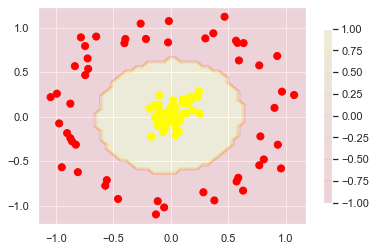
\includegraphics[width=\linewidth]{../catalogue/select-04.png}
  \captionof{figure}{Visualisation of the decision boundary of a SVM.}
  \label{fig:svm}
\end{minipage}

% is the data from the training or testing set?
% what is the info obtained from the visualisation?
% what is the assertion doing? what is the info obtained here?
% does the assertion reflect the info obtained from the visualisation?

Figure~\ref{fig:svm} presents a visualisation obtained from a notebook that performs binary classification using Support Vector Machines (SVM). The model is trained on the \texttt{make\_circles}~\footnote{REFME} dataset obtained from scikit-learn~\footnote{REFME}. The visualisation shows the two classes present in the training set, and the decision boundary of the model.

Listing~\ref{lst:svm} shows the corresponding assertion that was defined below Figure~\ref{fig:svm} in the notebook. The assertion checks if the model accuracy is above a threshold specified by the author of the notebook.

% NOTE it seems wrong that the visualisation is on the training set but the assertion is on the test set; but at the same time, it does seem "natural" to visualise the training set and calculate accuracy on the test set?

\subsection{Input Image, \texttt{predict\_proba}}

Figures~\ref{fig:football} and~\ref{fig:tennisball} are obtained from a notebook that uses a pre-trained image classifier from GluonCV library~\footnote{https://cv.gluon.ai}, to identify images that contain tennis balls.

Listing~\ref{lst:football} presents the assertion related to Figure~\ref{fig:football}. The assertion checks if the probability estimate of the model for the given input image, is close to the specified value with a precision of up to three decimal places. Since the model is trained to detect tennis ball, and the input image is of a football, the specified probability estimate is very low.

\begin{minipage}{0.5\textwidth}
  \begin{lstlisting}[language=Python]
np.testing.assert_almost_equal(pred_proba, 2.0355723e-05, decimal=3)
  \end{lstlisting}
  \captionof{lstlisting}{Assertion to check if the probability estimate of the model is close to the specified value. The input image is of a football. Since the model is trained to detect tennis balls, the specified value is very small.}
  \label{lst:football}
\end{minipage}
\begin{minipage}{0.5\textwidth}
  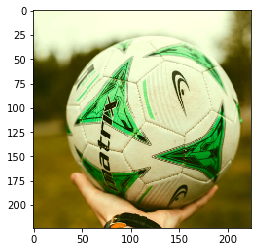
\includegraphics[width=\linewidth]{../catalogue/select-35a.png}
  \captionof{figure}{Random Input image of a football from the test set.}
  \label{fig:football}
\end{minipage}

In contrast, Listing~\ref{lst:tennisball} specifies a much higher probability estimate since the input image contains tennis balls.

\begin{minipage}{0.5\textwidth}
  \begin{lstlisting}[language=Python]
np.testing.assert_almost_equal(pred_proba, 0.9988895, decimal=3)
  \end{lstlisting}
  \captionof{lstlisting}{Assertion to check if the probability estimate of the model is close to the specified value. Compared to Figure~\ref{fig:football}, the specified value is much higher, since the input image is of tennis balls.}
  \label{lst:tennisball}
\end{minipage}
\begin{minipage}{0.5\textwidth}
  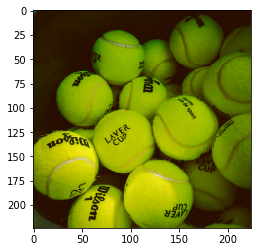
\includegraphics[width=\linewidth]{../catalogue/select-35b.png}
  \captionof{figure}{Random input image of tennis balls from the test set.}
  \label{fig:tennisball}
\end{minipage}

\subsection{Training loss}

% TODO this is also a condition0 example, the NB was flagged for another viz,assert pair that is not relevant to us. How do we handle this? Because this is a really nice example to have!
Figure~\ref{fig:loss-relaxed} shows the loss of a Recurrent Neural Network (RNN) over the trainin epochs. The visualisation was obtained from a notebook that trains an RNN to generate human names.

\begin{minipage}{0.5\textwidth}
  \begin{lstlisting}[language=Python]
assert np.mean(history[:10]) >np.mean(history[-10:]), "RNN didn't converge"
  \end{lstlisting}
  \captionof{lstlisting}{Assertion to check that the mean of first 10 observations of training loss is higher than the mean of last 10 observations. In other words, the assertion checks that the loss decreased after training and the model converged to an optimal minima.}
  \label{lst:loss-relaxed}
\end{minipage}
\begin{minipage}{0.5\textwidth}
  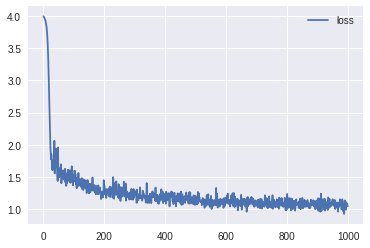
\includegraphics[width=\linewidth]{../catalogue/select-12.png}
  \captionof{figure}{Loss over training epochs of an ML model.}
  \label{fig:loss-relaxed}
\end{minipage}

\begin{minipage}{0.5\textwidth}
  \begin{lstlisting}[language=Python]
# assert we actually descended at each step
for i in range(1, n_steps):
    assert loss_array_true_grad[i] - loss_array_true_grad[i-1]) <= 0
  \end{lstlisting}
  \captionof{lstlisting}{Assertion to check that the loss at each iteration $n$ is less than or equal to the loss at $n-1$.}
  \label{lst:loss-strict}
\end{minipage}
\begin{minipage}{0.5\textwidth}
  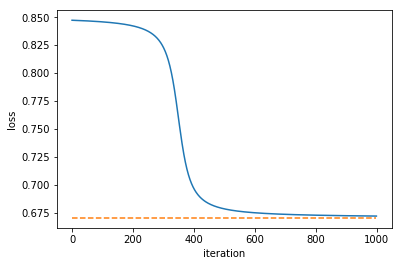
\includegraphics[width=\linewidth]{../catalogue/select-267.png}
  \captionof{figure}{Another example of the same visualisation presented in Figure~\ref{fig:loss-relaxed}. The visualisation shows the training loss of an ML model over time.}
  \label{fig:loss-strict}
\end{minipage}

\subsection{Coefficient of Determination}

Figure~\ref{fig:r2} shows a visualisation obtained from a notebook that trains a RNN to predict the levels of Nitrogen Dioxide ($NO_2$) in the next 24 hour window. The model is trained using time-series data consisting of historical readings of $NO_2$ and meteorological data such as temparate, humidity, wind speed, and such.

% I want to say that the spread of the points should be close to the diagonal to indicate a good fit which is not the case here.
The visualisation shows a scatterplot of the real and predicted values of $NO_2$ from the test set. The scatterplot shows a linear relationship between the ground truth and predictions indicating that the model learned something during training. However, the spread of the points is wide indicating that it can be improved with more fine tuning.

Listing~\ref{lst:r2} presents the corresponding analytical test which was defined below Figure~\ref{fig:r2}. The Coefficient of Determination ($R^2$) is calculated using the \texttt{r2\_score} method from scikit-learn~\footnote{REFME}. The assertion checks that the $R^2$ is higher than a specified threshold.


\begin{minipage}{0.5\textwidth}
  \begin{lstlisting}[language=Python]
r2_gru = r2_score(y_test, y_pred)
assert r2_gru > 0.6
  \end{lstlisting}
  \captionof{lstlisting}{Assertion to check that the Coefficient of Determination ($R^2$) is higer than the specified threshold.}
  \label{lst:r2}
\end{minipage}
\begin{minipage}{0.5\textwidth}
  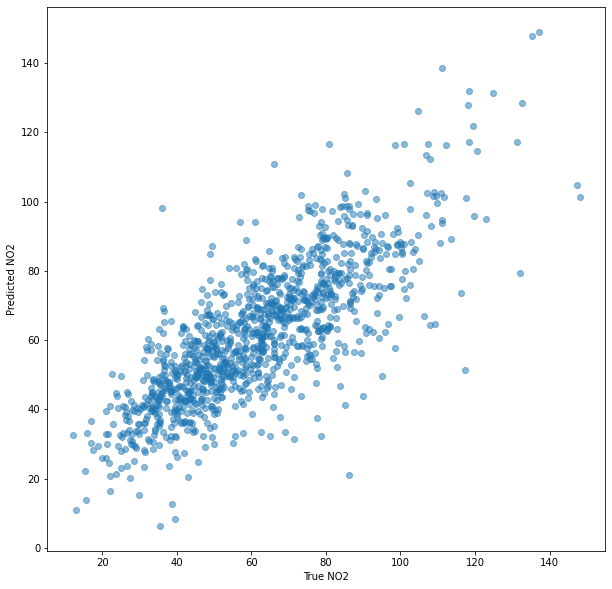
\includegraphics[width=\linewidth]{../catalogue/select-332a.png}
  \captionof{figure}{Scatterplot of the actual and predicted labels of a dataset. The visualisation shows that there is a linear relationship between the true and predicted labels.}
  \label{fig:r2}
\end{minipage}

\subsection{Time-series Prediction}

% TODO this is condition0! find an alternative!

\begin{minipage}{0.5\textwidth}
  \begin{lstlisting}[language=Python]
# Result of the wfc function for the best choice of s
assert np.isclose(best_wfv, 7685.546728971963, 0.001)
  \end{lstlisting}
\end{minipage}
\begin{minipage}{0.5\textwidth}
  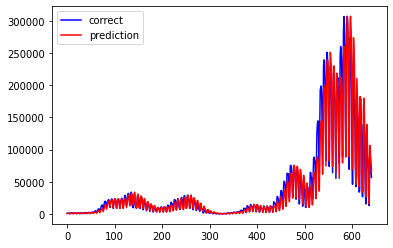
\includegraphics[width=\linewidth]{../catalogue/select-117b.png}
\end{minipage}

\section{Discussion}\label{sec:discuss}
% NOTE comment on the over-whelming presence of magic thresholds in ML testing! where are authors getting these numbers from? link this to requirements engineering?

% NOTE comment on the anti-patterns in testing that we observe in the 5 patterns presented

% NOTE link the qualitative and quantitative testing to the ML lifecycle: how some tests will let practitioner know when something changes

% NOTE comment on evolution? we have to look at the entire lifecycle of a visualisation: notebooks are run iteratively?
\section{Threats to Validity}\label{sec:threats}
% defend use of github as source for notebooks:
% - why did kaggle not work (refer to notes)
% - why did the existing replication packages not work?

% motivation for keeping the search on github broad:
% - not only does it pick up python assert statements, but also flags
% - notebooks that use other testing libraries or modules that provide a
% - testing interface. This is a good compromise between doing an
% - exhaustive search of all testing method names in the python
% - ecosystem and then doing a search for each of those patterns
\section{Conclusion}\label{sec:conclude}

\bibliographystyle{ACM-Reference-Format}
\bibliography{bibliography}
\end{document}

